\documentclass{beamer}
\usepackage[utf8]{inputenc}
\usepackage[T2A]{fontenc}
\usepackage[english, russian]{babel}
%\usepackage[sfdefault, light]{roboto}
\usepackage{epstopdf}
\usepackage[font={footnotesize}, labelfont={footnotesize}]{caption}
\usepackage[font={footnotesize}, labelfont={footnotesize}]{subcaption}
\usepackage{bm}
\usepackage[absolute,overlay]{textpos}
  \setlength{\TPHorizModule}{1mm}
  \setlength{\TPVertModule}{1mm}

\usepackage{tikz}

% Listings
\usepackage{listings}
\definecolor{codegreen}{rgb}{0,0.6,0}
\definecolor{codegray}{rgb}{0.5,0.5,0.5}
\definecolor{codepurple}{rgb}{0.58,0,0.82}
\definecolor{backcolour}{rgb}{0.95,0.95,0.92}
 
\lstdefinestyle{pythonstyle}{
    backgroundcolor=\color{backcolour},   
    commentstyle=\color{codegreen},
    keywordstyle=\color{magenta},
    numberstyle=\tiny\color{codegray},
    stringstyle=\color{codepurple},
    basicstyle=\scriptsize,
    breakatwhitespace=false,         
    breaklines=true,                 
    captionpos=b,                    
    keepspaces=true,                 
    numbers=left,                    
    numbersep=5pt,                  
    showspaces=false,                
    showstringspaces=false,
    showtabs=false,                  
    tabsize=2
}
\lstset{style=pythonstyle, language=Python}

\graphicspath{ {images/} }
\setbeamertemplate{caption}{\raggedright\insertcaption\par}
\def\figurename{}

\title{Базовые модели машинного обучения:\\k-ближайших соседей}
\date[\today]{Практика по дисциплине <<Технологии ИИ>>\\\today}
\author[Anton]{Гирдюк Дмитрий Викторович\\Першин Антон Юрьевич, Ph.D.\\Никольская Анастасия Николаевна}

\institute{Программа <<Большие данные и распределенная цифровая платформа>>\\Санкт-Петербургский государственный университет}

\usetheme{tonythequick}


\begin{document}

\begin{frame}
\titlepage
\end{frame}

\setcounter{framenumber}{0}

\section{}

\begin{frame}{Метод $k$-ближайших соседей}
    \small

    \begin{itemize}
        \item Метод $k$-ближайших соседей ($k$-nearest neighbors, kNN) -- относительно простой метрический алгоритм для задач классификации, основанный на оценке схожести некоторого наблюдения/объекта/сэмпла и классифицированных ранее его соседей.
        \item Классифицируемое наблюдение относится к классу, преобладающему среди $k$ ближайших соседей наблюдения.
        \item Близость определяется некоторой фиксированной метрикой (например, евлкидовой).
        \item Основное предположение заключается в том, что близкие наблюдения (в смысле значения метрики) принадлежат одному классу (так называемая <<гипотеза компактности>>).
    \end{itemize}
\end{frame}

\begin{frame}{Пример}
    \small
    \begin{figure}[H]
        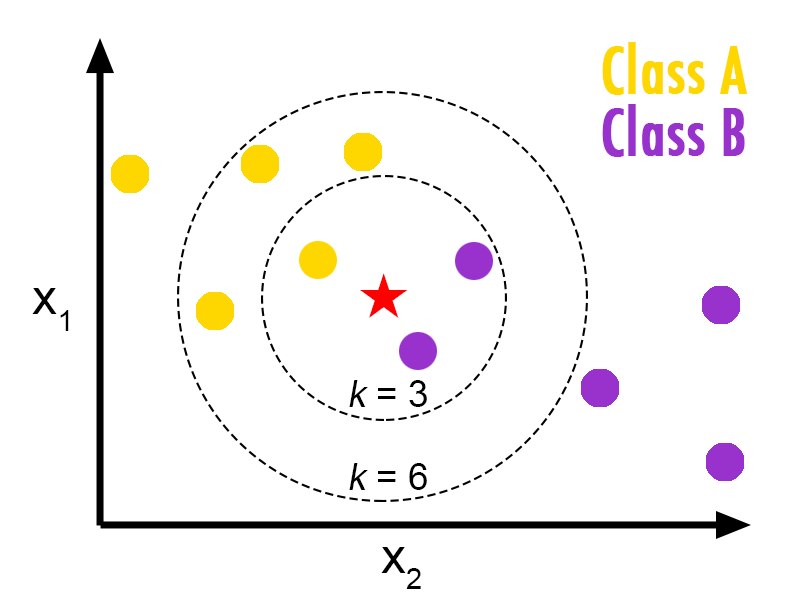
\includegraphics[width=0.8\textwidth]{images/knn_viz.png}
    \end{figure}
    \href{https://gist.github.com/wanibal84/e8c15faa69081dc0c68d79d5cdb12398}{Источник изображения}
\end{frame}

\begin{frame}{Формальное определение}
    \small
    \begin{itemize}
         \item Имеем размеченную обучающую выборку $X = \{ x_i\}_{i=1}^n, Y = \{ y_i \}, x_i \in \mathbb{R}^m, y_i \in \mathbb{N}$.
         \item Выберем некоторую метрику $\rho(x_i, x_j)$.
         \item Отсортируем для некоторого нового наблюдения $\widehat x$ объекты обучающей выборки $X$:
         $$\rho(\widehat x, x_{o_1}) \leqslant \rho(\widehat x, x_{o_2}) \leqslant \ldots \leqslant \rho(\widehat x, x_{o_n})$$
    \end{itemize}
\end{frame}

\begin{frame}{Формальное определение (2)}
    \small
    \begin{itemize}
        \item Тогда метод ближайших соседей формально записывается в виде
         $$\widehat y = \arg \max_{y \in Y} \sum_{i=1}^n \left [ y_{o_i} = y \right ] \omega(i, \widehat x),$$
         где $\omega(i, \widehat x)$ есть весовая функция, которая оценивает степень важности $o_i$-го наблюдения для классификации $\widehat x$.
        \item $\omega(i, \widehat x) = [ i = 1 ]$ -- метод ближайшего соседа.
        \item $\omega(i, \widehat x) = [ i \leqslant k ]$ -- метод k-ближайших соседей.
    \end{itemize}
    
\end{frame}

\begin{frame}{Выбор $k$}
    \small
    \begin{itemize}
        \item Очевидно, что при $k = 1$ метод является неустойчивым к выбросам, а при $k = n$ все новые наблюдения будут относиться к наиболее частотному классу.
        \item На практике $k$ выбирается либо на основе внешних свойств исследуемой области, либо путем кросс-валидации.
    \end{itemize}
\end{frame}

\begin{frame}{Типы наблюдений}
    \small
    \begin{itemize}
        \item Наблюдения можно разделить на 3 типа.
        \item Эталоны -- самые информативные наблюдения, типичные представители своего класса. 
        \item Когда в некоторой области признакового пространства содержится большое количество эталонных наблюдений, многие из них становятся неинформативными: удалив их, это никоим образом не скажется на качестве классификации.
        \item Наконец, выбросы. Под ними понимаются как наблюдения, достаточно далеко удаленные ото всех остальных, так и те, что находятся в пределах большого числа наблюдений другого класса.
        \item Понятно, что чем меньше в обучающей выборке неинформативных наблюдений и выбросов, тем лучше качество классификации.
    \end{itemize}
\end{frame}

\begin{frame}{Масштабируемость}
    \small
    \begin{itemize}
        \item Чем больше обучающая выборка, тем дольше происходит классификация.
        \item Если в решаемой задаче необходимо последовательное дообучение, вычисление расстояния до всех наблюдений становится весьма неэффективным.
        \item В таком случае, необходимы эффективные реализации поиска соседей на основе специфических структур данных/индексов (например, KD-деревья), или вовсе специальные схемы аппроксимации (например, Hierarchical Navigable Small Worlds, HNSW).
    \end{itemize}
\end{frame}

\begin{frame}{Выбор $rho$}
    \small
    \begin{itemize}
        \item Метрика должна достаточно адекватно отражать схожесть наблюдений в признаковом пространстве. Проблема состоит в том, что понятие "адекватно" сложно формализовать.
        \item Числовые признаки практически всегда необходимо нормализовывать. Иначе вклад одних будет затмевать другие. С другой стороны, некоторые признаки могут быть куда более значимыми, чем другие. 
        \item Проклятие размерности тоже никто не отменял. Если признаков много, то сумма отклонений между компонентами двух наблюдений приведет к тому, что большинство наблюдений будут равноудалены относительно друг друга (см. закон больших чисел). Зато можно брать произвольное $k$!
    \end{itemize}
\end{frame}

\begin{frame}{Выбор $rho$ (2)}
    \small
    \begin{itemize}
        \item Отсюда следует, что либо признаки следует каким-либо образом отбирать, либо задавать им в метрике весовые коэффициенты. Или вовсе <<обучать метрику>> (см. metric learning) под признаковое пространство.
    \end{itemize}
\end{frame}

\begin{frame}{Обсуждение}
    \small

    \begin{itemize}
        \item Метод $k$-ближайших соседей, наряду с деревьями, отличное базовое решение.
        \item kNN имеет всего 2 гиперпараметра, каждый из которых имеет принципиальное значение.
        \item Как и деревья решений, обобщается на задачи регрессии: значение вычисляется как среднее значений по соседям.
    \end{itemize}
\end{frame}

\begin{frame}{$kNN$ в scikit-learn}
    \small

    \begin{itemize}
        \item kNN реализован в scikit-learn: KNeighborsClassifier и KNeighborsRegressor. \item Есть поддержка разреженных данных. 
        \item Кроме числа соседей $k$ можно задавать следующее:
        \begin{itemize}
            \item weights, веса наблюдений. Либо равнозначны (дефолтное), либо с учетом расстояния до соседей.
            \item algorithm. Способ поиска соседей: брутфорс, ball-дерево, KD-дерево, и автоматический подбор подходящего с учетом обучающей выборки (дефолтное).
            \item leaf\_size. Максимальный размер листа в дереве, если выбрано ball/KD-дерево.
            \item metric и $p$. Метрику можно как реализовать самостоятельно, так и использовать из имеющегося: Минковского ($p$ -- ее параметр) и ее частные случаи (Чебышева и Манхэттенская).
        \end{itemize}
    \end{itemize}
\end{frame}


\end{document}
